\nsection{OSN 3 Основные сведения об объектном языке ограничений (OCL): состав OCL выражения, навигация по ассоциациям, виды коллекций, операции с коллекциями, учёт наследования в выражениях и наследование ограничений. Примеры использования OCL.}

\textbf{Ограничение} (constraint) – условие, накладываемое на значения одного или нескольких
элементов модели. Ограничение не является инструкцией или командой, которую следует выполнить,
оно формулируется как утверждение, которое должно быть истинным. Элемент модели - объект, или класс, или пакет, или подсистема, или атрибут, или операция, или связь.
Необходим формальный язык, который не допускает произвольных толкований и имеет стандартный синтаксис и семантику (воизбежание неправильных трактовок). 

\textbf{OCL (Object Constraint Language)} – это текстовый (\textit{невизуальный}) язык описания ограничений. OCL язык со строгой типизацией. OCL декларативный язык (для ограничений не определяется конкретная процедура их проверки). Никакое OCL-ограничение не меняет состояния элементов модели, не добавляет в модель новых элементов, не удаляет элементы из модели, у ограничения нет побочных эффектов. OCL может быть использован для формулирования запросов, возвращающих целое значение, вещественное, строку, объект, коллекцию и т. п.. При этом, не определяется способ вычисления этого запроса. OCL-запрос не обязательно при вычислении вернёт булеву величину, поэтому от понятия ограничения перейдём к более общему понятию – OCL-выражению.
Синтаксис OCL-выражения
\begin{verbatim}
<OCL-выражение> ::=
  <указание контекста>
  [(inv|pre|post|body|init|derive|def):<тело выражения>]
\end{verbatim}

В записи использованы символы языка БНФ: <> выделяют нетерминалы, ( | ) –вхождение одной
из указанных альтернатив, [] вхождение 1 или более раз, {} – вхождение 0 или более раз. Терминалы
записаны жирным шрифтом.
\textbf{Контекст}. В любом OCL-выражении указывается определенный контекст. Как правило,
контекстом является элемент модели (класс, класс ассоциации, интерфейс и т.п.), с которым связано
ограничение.
\begin{verbatim}
    <указание контекста> ::= context <имя элемента модели>
\end{verbatim}

Для того чтобы сослаться на произвольный экземпляр контекста в теле выражения используется
слово self. Чтобы много раз не писать self, оно часто опускается. По смыслу self аналогично this в C++.

Классификация ограничений:
\begin{itemize}
    \item Инвариант класса, который всегда справедлив для всех экземпляров класса (inv:)
    \item Предусловие операции, которое должно быть истинно перед выполнением операции (pre:)
    \item Постусловие операции, истинное всегда после выполнения операции (post:).
    \item Тело запроса – описание результата операции-запроса (body:)
    \item Начальное значение атрибута (init:)
    \item Правило вывода, описывающее производные атрибуты, ассоциации или классы (derive:).
    \item Дополнительное выражение, введённое для удобства записи других ограничений (def:).
\end{itemize}

В теле выражения используются \textit{boolean}, \textit{integer}, \textit{string}, \textit{real} (а также \textit{xor}, \textit{implies} и тд и тп)

\begin{verbatim}
<условное выражение> ::=
if <логическое выражение> then <выражение>
else <выражение>
endif    
\end{verbatim}

В телах OCL-выражений используются типы и имена (классов, атрибутов, операций) из модели.

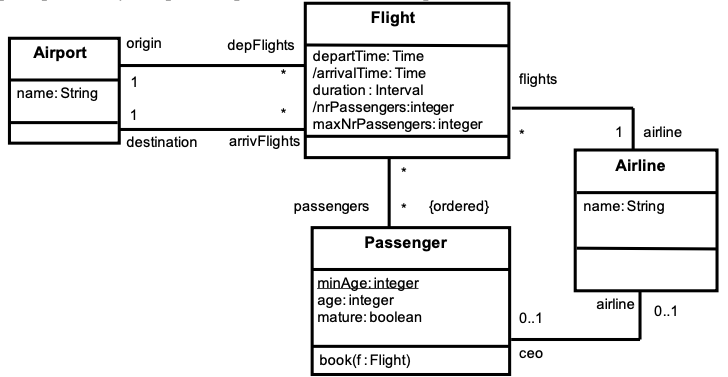
\includegraphics[scale=0.37]{pics/ocl.png}

\textbf{context Flight inv: self.maxNrPassengers <= 1000}   – в любом рейсе максимальное количество пассажиров не превышает 1000 (использован атрибут объекта – экземпляра класса Flight).

\textbf{context Flight:maxNrPassengers:Integer init: 1000} – в любом рейсе максимальное количество
пассажиров по умолчанию = 1000

\begin{verbatim}
context Flight
inv: self.origin <> self.destination
inv: self.origin.name = ‘Amsterdam’
\end{verbatim}

У любого рейса аэропорт назначения и аэропорт вылета не совпадают, а также аэропорт вылета называется ‘Amsterdam’

При навигации по связям, если на другом конце указана мощность связи *, от одного объекта мы приходим к нескольким связанным с ним (например, один аэропорт является аэропортом вылета для нескольких рейсов), поэтому в OCL введено понятие \textbf{коллекции}. Коллекции могут состоять либо из объектов, либо из элементов простых типов, либо из элементов типов, определенных в модели, либо из коллекций. Виды коллекций:
\begin{itemize}
    \item \textbf{Set} (множество– неупорядоченный набор без повторов) – для экземпляра класса Airport прибывающие рейсы составляют множество объектов Flight.
    \item \textbf{Bag} (неупорядоченный набор с повторами) – для экземпляра класса Airport количества пассажиров на каждом из прибывающих рейсов составляют bag целочисленных значений. 
    \item \textbf{OrderedSet} (упорядоченный набор без повторов) – для экземпляра класса Flight все его пассажиры составляют orderedSet объектов Passenger.
    \item \textbf{Sequence} (упорядоченный набор с повторами) – для экземпляра класса Flight возрасты всех его пассажиров составляют sequence целочисленных значений. 
\end{itemize}

Операция \textbf{collect()} возвращает коллекцию значений, полученных при вычислениях выражения
для всех элементов коллекции. (\textbf{context Airport inv: self.arrivingFlights -> collect(airLine) -> notEmpty()} - $\forall$ аэропорта множество авиакомпаний, выполняющих прибывающие рейсы, не пусто.)

Операция \textbf{select()} возвращает совокупность тех элементов коллекции, для которых <выражение>
истинно. (\textbf{context Airport inv: self.departingFlights->select(duration<4)->notEmpty()} - $\forall$ аэропорта есть хоть один отправляющийся рейс длительностью менее 4 часов.). Аналог - \textbf{reject()}, который удаляет из коллекции все элементы, удовлетворяющие критерию отбора.

Операция \textbf{forAll()} возвращает true если <выражение> истинно для всех элементов коллекции, в
остальных случаях возвращается false. (\textbf{context Airport inv: self.departingFlights->forAll(maxNrPassengers < 1000)} - $\forall$ аэропорта - у любого отправляющегося рейса максимальное количество пассажиров < 1000)

Операции над коллекциями:
\begin{itemize}
    \item isEmpty(): истина, если коллекция пуста, иначе – ложь;
    \item notEmpty(): истина, если коллекция не пуста, иначе – ложь;
    \item size(): количество элементов коллекции; self.departingFlights->size()
    \item sum(): сумма элементов коллекции; self.departingFlights.nrPassengers->sum()
    \item min(): минимальный элемент коллекции чисел;
    \item max(): максимальный элемент коллекции чисел;

\end{itemize}

При \textbf{наследовании} ограничений работает принцип подстановки БарбарыЛисковы: «Где может находиться экземпляр суперкласса, туда всегда может быть подставлен экземпляр его любого подкласса.» \begin{itemize}
    \item Инвариант суперкласса наследуется любым подклассом и может быть усилен в подклассе, но не
ослаблен.
    \item Предусловие операции может быть ослаблено в подклассе или оставлено прежним, как в суперклассе, но не может быть усилено.
    \item Постусловие операции может быть усилено в подклассе или оставлено прежним, как в суперклассе, но не может быть ослаблено.
\end{itemize}
Если в ограничении требуется проверить, конкретный тип экземпляра, то используют стандартную операцию \textbf{ocllsTypeOf(<тип>)}

